\documentclass[]{AVSSimReportMemo}
\usepackage{AVS}

\newcommand{\ModuleName}{velocityPointing}
\newcommand{\subject}{Guidance Module for Velocity Axis Pointing}
\newcommand{\status}{Initial Version}
\newcommand{\preparer}{M. Cols}
\newcommand{\summary}{Generate the attitude reference to perform a constant pointing towards a Velocity orbit axis}


\begin{document}

\makeCover


%
% enter the revision documentation here
% to add more lines, copy the table entry and the \hline, and paste after the current entry.
%
\pagestyle{empty}
{\renewcommand{\arraystretch}{2}
\noindent
\begin{longtable}{|p{0.5in}|p{4.5in}|p{1.14in}|}
\hline
{\bfseries Rev}: & {\bfseries Change Description} & {\bfseries By} \\
\hline
Draft & initial copy & M. Cols \\
\hline

\end{longtable}
}

\newpage
\setcounter{page}{1}
\pagestyle{fancy}

\tableofcontents
~\\ \hrule ~\\

\begin{figure}[htb]
  \centerline{
  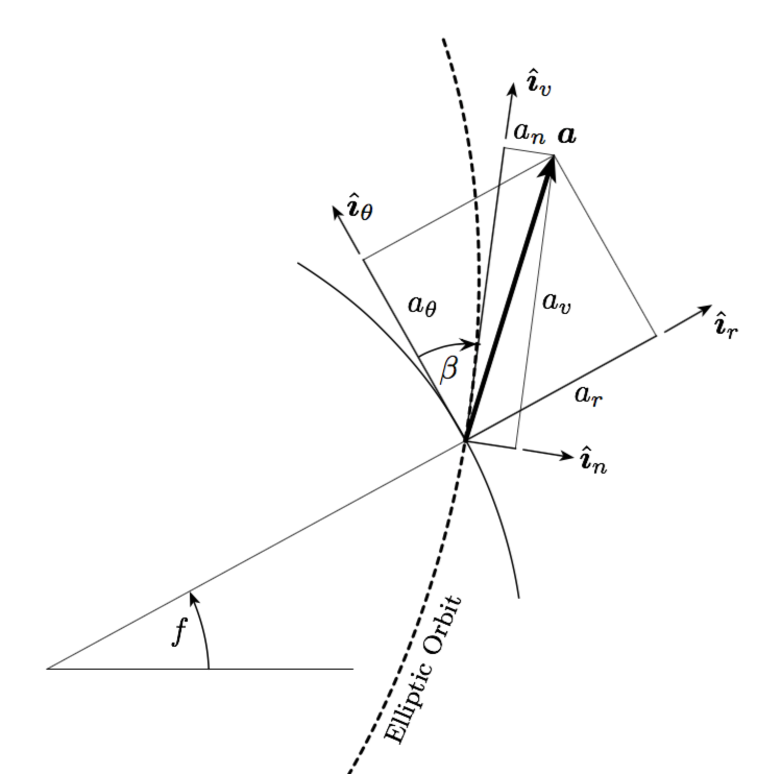
\includegraphics[width=7cm]{Figures/velocityPoint}
  }
  \caption{Illustration of the planet orbit frames, Hill $\mathcal{H}$ and Velocity $\mathcal{V}$.}
  \label{fig:Fig1}
\end{figure}

\section{Reference Frame Definition}
The velocity frame is defined as $\mathcal{V}:\{ \hat{\bm\imath}_{n}, \hat{\bm\imath}_{v}, \hat{\bm\imath}_{h} \}$ as illustrated in Figure~\ref{fig:Fig1}.  Here $\hat{\bm\imath}_{v}$ is aligned with the orbit velocity direction, $\hat{\bm\imath}_{h}$ is aligned with the orbit normal direction and $\hat{\bm\imath}_{n}$ is the normal vector that completes a right-handed coordinate frame.  On the other hand, the  Hill orbit frame is defined as $\mathcal{O}:\{\hat{\bm\imath}_{r}, \hat{\bm\imath}_{\theta}, \hat{\bm \imath}_{h}  \}$.\par  
These two frames differ by a 3-axis rotation with the angle $-\beta$.  In terms of $\beta$, the $[VH]$ DCM to map from $\mathcal{H}$ to $\mathcal{V}$ is given by
\begin{equation}
  \label{eq:VHbeta}
  [VH] = [M_{3}(-\beta)] = \begin{bmatrix}
    \cos\beta & -\sin\beta & 0 \\
    \sin\beta & \cos\beta &0 \\
    0 & 0 & 1
  \end{bmatrix}
\end{equation}

\section{Velocity Frame Rate Development}
Next the Velocity frame rate $\dot\beta$ relative to the orbit frame is determined.
Note the following identities:
\begin{equation}
  \label{eq:tanbeta}
  \tan\beta = \frac{e \sin f}{1 + e \cos f}
\end{equation}
\begin{equation}
  \label{eq:cos2beta}
  \cos^{2}\beta^{} = \frac{(1+e \cos f)^{2}}{1+e^{2}+2 e \cos f}
\end{equation}
Taking the derivative of Eq.~\eqref{eq:tanbeta} yields
\begin{equation}
  \label{eq:dbeta}
  \dot\beta =   \frac{ e (e+\cos f)}{1+e^{2}+2 e \cos f} \dot f
\end{equation}
To find the relative angular acceleration $\ddot\beta$, Eq.~\eqref{eq:dbeta} is differentiated again.
\begin{equation}
  \label{eq:ddbeta}
  \ddot\beta = 
   \frac{e(e+\cos f)}{1+e^{2}+2 e \cos f} \ddot f
   +\frac{
  e  (e^{2}-1)\sin f
  }{
  (1+e^{2}+2 e \cos f)^{2}
  } \dot f^{2}
\end{equation}


\section{Angular Velocity Vectors}
Next, let us evaluate the Velocity frame angular velocities.  As both the $\mathcal{V}$ and $\mathcal{H}$ frame rotate about the common $\hat{\bm\imath}_{h}$ axis, note that
\begin{align}
  \bm\omega_{V/H} &= -\dot\beta \hat{\bm\imath}_{h}
  \\
  \bm\omega_{H/N} &= \dot f \hat{\bm\imath}_{h}
\end{align}
This leads to
\begin{equation}
  \label{eq:omegaVN}
  \bm\omega_{V/N} = \bm\omega_{V/H} + \bm\omega_{H/N} = 
  \frac{1+e \cos f}{1+e^{2} + 2 e \cos f} \dot f \hat{\bm\imath}_{h}
\end{equation}
Similarly, we find
\begin{equation}
  \label{eq:domegaVN}
  \dot{\bm\omega}_{V/N} = \dot{\bm\omega}_{V/H} + \dot{\bm\omega}_{H/N} = 
  \left( \frac{1+e\cos f}{1+e^{2}+2 e \cos f} \ddot f
  - \frac{
  e  (e^{2}-1)\sin f
  }{
  (1+e^{2}+2 e \cos f)^{2}
  } \dot f^{2} \right) \hat{\bm\imath}_{h}
\end{equation}

The orbit frame angular rates and accelerations are determined through the standard astrodynamics relations:
\begin{align}
  \dot f &= \frac{h}{r^{2}}
  \\
  \ddot f &= - \frac{\mu e \sin f}{r^{3}}
\end{align}


\bibliographystyle{unsrt}
\bibliography{references}

\end{document}
